\section{Related Work}
\label{sec:related}

\subsection{Haskell}
\label{sec:haskelldesc}

Haskell is a convenient choice for our purposes for several reasons. Here we discuss the relevant language features from a high-level:

\begin{description}

\item{Functional}: All control flow is performed by function abstraction and application, which we can reason about using standard rules of inference such as \emph{modus ponens}.

\item{Pure}: Execution of actions (e.g. reading files) is separate to evaluation of expressions; hence our reasoning can safely ignore complicated external and non-local interactions.

\item{Statically Typed}: Expression are constrained by \emph{types}, which can be used to eliminate unwanted combinations of values, and hence reduce search spaces; \emph{static} types can be deduced syntactically, without having to execute the code.

\item{Non-strict}: If an evaluation strategy exists for $\beta$-normalising an expression (i.e. performing function calls) without diverging, then a non-strict evaluation strategy will not diverge when evaluating that expression. This is rather technical, but in simple terms it allows us to reason effectively about a Turing-complete language, where evaluation may not terminate. For example, when reasoning about \emph{pairs} of values \hs{(x, y)} and projection functions \hs{fst} and \hs{snd}, we might want to use an ``obvious'' rule such as $\forall \text{\hs{x y}}, \text{\hs{x}} = \text{\hs{fst (x, y)}}$. Haskell's non-strict semantics makes this equation valid; whilst it would \emph{not} be valid in the strict setting common to most other languages, where the expression \hs{fst (x, y)} will diverge if \hs{y} diverges (and hence alter the semantics, if \hs{x} doesn't diverge).

\item{Algebraic Data Types}: These provide a rich grammar for building up user-defined data representations, and an inverse mechanism to inspect these data by \emph{pattern-matching}. For our purposes, the useful consequences of ADTs and pattern-matching include their amenability for inductive proofs and the fact they are \emph{closed}; i.e. an ADT's declaration specifies all of the normal forms for that type. This makes exhaustive case analysis trivial, which would be impossible for \emph{open} types (for example, consider classes in an object oriented language, where new subclasses can be introduced at any time).

\item{Parametricity}: This allows Haskell \emph{values} to be parameterised over \emph{type-level} objects; provided those objects are never inspected. This has the \emph{practical} benefit of enabling \emph{polymorphism}: for example, we can write a polymorphic identity function \hs{id :: forall t. t -> t}. \footnote{Read ``\hs{a :: b}'' as ``\hs{a} has type \hs{b}'' and ``\hs{a -> b}'' as ``the type of functions from \hs{a} to \hs{b}''.} Conceptually, this function takes \emph{two} parameters: a type \hs{t} \emph{and} a value of type \hs{t}; yet only the latter is available in the function body, e.g. \hs{id x = x}. This inability to inspect type-level arguments gives us the \emph{theoretical} benefit of being able to characterise the behaviour of polymorphic functions from their type alone, a technique known as \emph{theorems for free} \citep{wadler1989theorems}.

\item{Type classes}: Along with their various extensions, type classes are interfaces which specify a set of operations over a type (or other type-level object, such as a \emph{type constructor}). Many type classes also specify a set of \emph{laws} which their operations should obey but, lacking a simple mechanism to enforce this, laws are usually considered as documentation. As a simple example, we can define a type class \hs{Semigroup} with the following operation and associativity law:

\begin{lstlisting}[language=Haskell, xleftmargin=.2\textwidth, xrightmargin=.2\textwidth]
op :: forall t. Semigroup t => t -> t -> t
\end{lstlisting}

$$\forall \text{\hs{x y z}}, \text{\hs{op x (op y z)}} = \text{\hs{op (op x y) z}}$$

The notation \hs{Semigroup t =>} is a \emph{type class constraint}, which restricts the possible types \hs{t} to only those which implement \hs{Semigroup}. \footnote{Alternatively, we can consider \hs{Semigroup t} as the type of ``implementations of \hs{Semigroup} for \hs{t}'', in which case \hs{=>} has a similar role to \hs{->} and we can consider \hs{op} to take \emph{four} parameters: a type \hs{t}, an implementation of \hs{Semigroup t} and two values of type \hs{t}. As with parameteric polymorphism, this extra \hs{Semigroup t} parameter is not available at the value level. Even if it were, we could not alter our behaviour by inspecting it, since Haskell only allows types to implement each type class in at most one way, so there would be no information to branch on.} There are many \emph{instances} of \hs{Semigroup} (types which may be substituted for \hs{t}), e.g. \hs{Integer} with \hs{op} performing addition. Many more examples can be found in the \emph{typeclassopedia} \citep{yorgey2009typeclassopedia}. This ability to constrain types, and the existence of laws, helps us reason about code generically, rather than repeating the same arguments for each particular pair of \hs{t} and \hs{op}.

\item{Equational}: Haskell uses equations at the value level, for definitions; at the type level, for coercions; at the documentation level, for typeclass laws; and at the compiler level, for ad-hoc rewrite rules. This provides us with many \emph{sources} of equations, as well as many possible \emph{uses} for any equations we might discover. Along with their support in existing tools such as SMT solvers, this makes equational conjectures a natural target for our investigation.

\item{Modularity}: Haskell has a module system, where each module may specify an \emph{export list} containing the names which should be made available for other modules to import. When such a list is given, any expressions \emph{not} on the list are considered \emph{private} to that module, and are hence inaccessible from elsewhere. This mechanism allows modules to provide more guarantees than are available just in their types. For example, a module may represent email addresses in the following way:

\begin{lstlisting}[language=Haskell, xleftmargin=.2\textwidth, xrightmargin=.2\textwidth, upquote=true]
module Email (Email(), at, render) where

data Email = E String String

render :: Email -> String
render (E u h) = u ++ "@" ++ h

at :: String -> String -> Maybe Email
at "" h  = Nothing
at u  "" = Nothing
at u  h  = Just (E u h)
\end{lstlisting}

The \hs{Email} type guarantees that its elements have both a user part and a host part (modulo divergence), but it does not provide any guarantees about those parts. We also define the \hs{at} function, a so-called ``smart constructor'', which has the additional guarantee that the \hs{Email}s it returns contain non-empty \hs{String}s. By ommitting the \hs{E} constructor from the export list on the first line \footnote{The syntax \hs{Email()} means we're exporting the \hs{Email} type, but not any of its constructors.}, the only way \emph{other} modules can create an \hs{Email} is by using \hs{at}, which forces the non-empty guarantee to hold globally.

\end{description}

Together, these features make Haskell code highly structured, amenable to logical analysis and subject to many algebraic laws. However, as mentioned with regards to type classes, Haskell itself is incapable of expressing or enforcing these laws (at least, without difficulty \citep{lindley2014hasochism}). This reduces the incentive to manually discover, state and prove theorems about Haskell code, e.g. in the style of interactive theorem proving (see \S \ref{sec:itp}), as these results may be invalidated by seemingly innocuous code changes. We will revisit the second-class status of theorem proving in Haskell in our discussion of theory exploration (\S \ref{sec:theoryexploration}), but we will remark that Haskell is thus in a unique position with regards to the discovery of interesting theorems. Namely that many discoveries may be available with very little work, simply because the code's authors are focused on \emph{software} development rather than \emph{proof} development. The same cannot be said, for example, of ITP systems; although our reasoning capabilities may be stronger in an ITP setting, much of the ``low hanging fruit'' will have already been found through the user's dedicated efforts, and hence TE would be more likely to fit into an automation role for the user, rather than providing truly unexpected new discoveries.

Other empirical advantages to studying Haskell, compared to either other programming languages or theorem proving systems, include:

\begin{itemize}

\item The large amount of Haskell code which is freely available online, e.g. in repositories like \href{http://hackage.haskell.org}{Hackage}, with which we can experiment.

\item The existence of conjecture generation and theory exploration systems for Haskell, such as \qspec{} and \hspec{}, and counterexample finders like \qcheck{}, \textsc{SmallCheck} and \textsc{SmartCheck}.

\item The remarkable amount of infrastructure which exists for working with Haskell code, including package managers, compilers, interpreters, parsers, static analysers, etc.

\end{itemize}

\iffalse

\subsection{Conjecture Generation}

The task of \emph{conjecture generation} lies at the heart of theory exploration, and

\subsubsection{Lemma generation}

\fi

\subsection{Exploration in Artificial Intelligence}

Theorem proving is not the only area of AI to have automation extended from problem \emph{solving} to problem \emph{invention}. Here we consider similar approaches in a variety of domains, and identify techniques which could be re-purposed in the context of theory exploration.

\subsubsection{Evolutionary Computation}

\emph{Evolutionary computation} is an umbrella term for heuristic search algorithms which mimic the process of evolution by natural selection among a population of candidate solutions \citep{back1997evolutionary}. Whilst \emph{genetic algorithms} are perhaps the most well-known instance of evolutionary computation, their use of \emph{strings} to represent solutions causes complications when comparing to a domain like theory exploration, where recursive structures of unbounded depth arise. Thankfully these problems are not insurmountable, for example \emph{genetic programming} can operate on tree-structures natively \citep{banzhaf1998genetic}, which makes evolutionary computation a useful source of ideas for reuse in our theory exploration setting.

Traditionally, evolutionary approaches assign solutions a \emph{fitness} value, using a user-supplied \emph{fitness function}. Fitness should correlate with how well a solution solves the user's problem; for example, the fitness of a solution to some engineering problem may depend on the estimated materials cost. If we frame the task of theory exploration in evolutionary computation terms, the fitness function would be our interestingness measure.

Pure exploration (i.e. for its own sake) has been studied in evolutionary computation for two main reasons: \emph{artificial life} and \emph{deceptive problems}. The former attempts to gain insight into the nature of life and biology through competition over limited resources. Whilst this may have utility in resource allocation, e.g. efficient scheduling of a portfolio of ATP programs, there is no direct connection to interestingness in theory exploration, so we will not consider it further (note that similar resource-usage ideas can also be found in the literature on \emph{artificial economies}, e.g. \citep{baum2000evolution}).

On the other hand, work on deceptive problems is highly relevant, as it has lead to studying various notions of intrinsic fitness, which are analogous to the interestingness measures we want. Deceptive problems are those where \textquote{pursuing the objective may prevent the objective from being reached} \citep{lehman2011abandoning}, which is caused by the fitness (objective) function having many local optima which are easy to find (e.g. by hill climbing), but few global optima which are hard to find. Many approaches try to avoid deception by augmenting the given fitness function to promote \emph{diversity} and \emph{novelty}, such as \emph{niching methods} \citep{sareni1998fitness}.

One example is \emph{fitness sharing}, which divides up fitness values between identical or similar solutions. Say we have a user-provided fitness function $f$, and a population containing two identical solutions $s_1$ and $s_2$; hence $f(s_1) = f(s_2)$. In a fitness sharing scheme, we interpret fitness as a fixed resource, distributed according to $f$; when multiple individuals occupy the same point in the solution space, they must \emph{share} the fitness available there. We can describe the fitness \emph{allocated} to a solution by augmenting $f$, e.g. if we allocate fitness uniformly between identical solutions we get:

$$f'(x) = \frac{f(x)}{\sum_{i=1}^n \delta_{s_i x}}$$

Where $n$ is the population size, $s_i$ is the $i$th solution in the population and $\delta$ is the Kronecker delta function. In the example above, assuming there are no other copies in the population, then $f'(s_1) = \frac{f(s_1)}{2} = \frac{f(s_2)}{2} = f'(s_2)$. By sharing in this way, the fitness of each solution is balanced against redundancy in the population: there may still be many copies of a solution, but only when the fitness is high enough to justify all of them.

There are many variations on this theme, such as sharing between ``close'' solutions rather than just identical ones and judging distance based on fitness (AKA phenotypically) rather than based on the location in solution space (AKA genetically). Yet the underlying principle is always the same: penalise duplication in order to promote diversity. This lesson can be carried over to our theory exploration context, where a theorem should be considered less interesting if it is ``close'' to others which have been found.

In a similar way, we can bias our search procedure, rather than our fitness function, towards diversity. The search procedure in population-based evolutionary algorithms consists of \emph{selecting} one or more individuals from the population, e.g. via truncation (select the best $n$ individuals, discarding the rest); then \emph{transforming} the selected individuals, e.g. via mutation and crossover, to obtain new solutions.

\newcommand{\argmin}{\operatornamewithlimits{argmin}}

Traditional selection methods are biased towards high fitness individuals (this is especially clear for truncation). Alternative schemes have been proposed which favour diversity \emph{at the expense of} fitness. For example, the fitness uniform selection scheme (FUSS) \citep{hutter2002fitness} selects a target fitness $f_t$ uniformly from the interval $\left[ f_{min}, f_{max} \right]$ between the highest and lowest of the population. An individual $s$ is then selected with fitness closest to $f_t$, i.e. $s = \operatornamewithlimits{argmin}\limits_{x} \lvert f(x) - f_t \rvert$

In this way, the fitness function $f$ is used to assign comparable quantities to solutions, but it is not treated as the objective; instead, the implicit objective is to maintain a diverse population, with individuals spread out uniformly in fitness space. This approach seems useful for informing our work in theory exploration, as it supports search criteria which \emph{describe} solutions, but which we may not want to \emph{optimise}. As a simple example, we might distinguish different forms of theorem by measuring how balanced their syntax trees are (-1 for left-leaning, +1 for right leaning, 0 for balanced); but it would be senseless to \emph{maximise} how far they lean.

Once we begin this process of augmenting fitness functions, or abandoning their use as objectives, an obvious question arises: what happens if our new function contains nothing of the original? This kind of pure exploration scenario leads to a variety of ideas for \emph{instrinsic} fitness, such as novelty \citep{lehman2011abandoning}, which can lead to learning useful ``stepping stones'' even in objective-driven domains. Such intrinsic notions of fitness are direct analogues of the interestingness measures we seek for theory exploration.

\subsubsection{Artificial Curiosity}
\label{sec:curiosity}

\begin{figure}
  \centering
  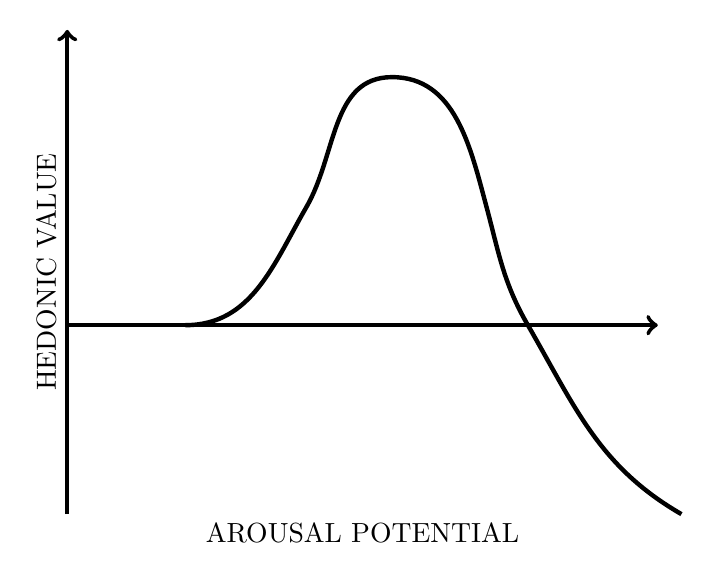
\begin{tikzpicture}[scale=0.75]
      % The image, for reference
      % \node[anchor=south west,inner sep=0] at (0,0) {\includegraphics[width=\textwidth]{wundt.png}};

      % Axes
      \draw[black,ultra thick,->] (1,0.8) -- (1,  9)   node[midway, above, sloped] {HEDONIC VALUE};     % y axis
      \draw[black,ultra thick,->] (1,4)   -- (11, 4);                                                   % x axis
      \path                       (1,0.8) -- (11, 0.8) node[midway, below]         {AROUSAL POTENTIAL}; % x axis label

      % Curve. The numbers come from tracing over wundt.png
      \draw[black,ultra thick] (3, 4)
           to[out=0,   in=240] (5.05, 6)
           to[out=60,  in=180] (6.5,  8.2)
           to[out=0,   in=105] (8.1,  6)
           to[out=-75, in=120] (8.8,  4)
           to[out=-60, in=150] (11.4, 0.8);

      % This version is closer, but a little jagged
      \iffalse
      \draw[black,ultra thick] (3, 4)
           to[out=0,   in=240] (5.05, 6)
           to[out=60,  in=225] (6,    8)
           to[out=45,  in=180] (6.5,  8.2)
           to[out=0,   in=135] (7.2,  8)
           to[out=-45, in=105] (8.1,  6)
           to[out=-75, in=120] (8.8,  4)
           to[out=-60, in=150] (11.4, 0.8);
      \fi
  \end{tikzpicture}

  \caption{The Wundt curve, reproduced from \citep{berlyne1970novelty}. The axes ``hedonic value'' and ``arousal potential'' are described as covering \textquote{reward value\dots preference or pleasure}, and \textquote{all the stimulus properties that tend to raise arousal, including novelty and complexity}, respectively.}

  \label{fig:wundt}
\end{figure}

\emph{Artificial curiosity} (AC) describes active learning systems which are rewarded based on how interesting the input or data they discover is \citep{schmidhuber2006developmental}. Although framed in the context of \emph{reinforcement learning}, this is clearly relevant to our theory exploration setting.

As an unsupervised learning task, AC has no access to labels or meanings associated with its input; the only features it can learn are the structure and relationships inherent in the data, which is very much what we would like a theory exploration system to do. The unifying principle of AC methods is to force systems away from inputs which are not amenable to learning; either because they are so familiar that there is nothing left to learn, or so unfamiliar that they are unintelligible. The resulting behaviour is characterised by the \emph{Wundt curve} (shown in figure \ref{fig:wundt}) \footnote{In practice, many measures avoid negative values for simplicity, in which cases we replace all negative points on the curve with zero.}, which has been used in psychology to explain human aesthetics and preferences \citep{berlyne1970novelty}.

We can divide AC approaches into two groups: the first, which we call \emph{explicit}, send inputs which follow a Wundt curve to their learning algorithm; the second, the \emph{implicit} approaches, instead modify the \emph{output} of their learning algorithm(s), such that the overall system follows a Wundt curve as an emergent property.

In the explicit case, the \emph{implicit reward} signals being learned are analogous to our notion of interestingness. A framework encompassing many examples is given in \citep{oudeyer2007intrinsic} in the context of reinforcement learning.

One particularly general measure is \emph{compression progress}: given a compressed representation of our previous observations, the ``progress'' is the space saved if we include the current observation. Observations which are incompressible or trivially compressible don't save any space, whilst observations which provide new information relevant to past experience can provide a saving. This can be translated to a theorem proving context very naturally: our observations are theorems and their proofs, whilst new theorems which generalise known results will allow us to compress their proofs.

% TODO: Examples
\citep{Schmidhuber1999}

Two sources of intrinsic reward are proposed in \citep{Hester.Stone:2012} for \emph{random forests}. A random forest is a population of decision trees, where each tree is trained on a sub-set of the available examples, each decision is made using a sub-set of the available features, and the predictions of every tree are averaged to obtain that of the forest \citep{randomforests}. The first intrinsic reward is the \emph{disagreement} between predictions; for a forest with $m$ models (trees), predicting features $x_1$ \dots $x_n$ of the state resulting from taking action $a$ in state $s$, we simply sum the Kullback-Leibler divergence $D_{\rm KL}$ of each prediction $P_1$ \dots $P_m$ from every other prediction:

\begin{equation}
  D(s,a) = \sum_{i = 1}^n \sum_{j = 1}^m \sum_{k = 1}^m D_{KL}(P_j(x_i|s,a) || P_k(x_i|s,a))
\end{equation}

$D(s,a)$ is an explicit AC reward, as it follows a Wundt curve as the complexity of transitions increases. For parts of the state space which have been fully learned, the models will agree on accurate predictions. For parts which are unlearnable, the models cannot infer any structure, and will converge to reporting the average of past observations; these predictions may not be accurate, but they will be in agreement. Hence it is the states which are amenable to learning which produce the largest disagreement.

The second intrinsic reward is simply a measure of distance from previous observations, which pushes the system towards unseen states regardless of how learnable they are (similar to the $R_{max}$ technique). This is too simple to meet our definition of AC, but it does force the models to generalise their predictions to unexplored states, acting to increase disagreement in the forest.

A key advantage of random forests is that their models are \emph{inspectable}: they not only give predictions, but also \emph{reasons} for those predictions (i.e. we can see which paths are taken through each decision tree). % TODO: The accuracy of these random forest models are compared

% TODO
\citep{Kaplan2006}
\citep{Lipson2007}
\citep{Luciw2011}
\citep{Macedo2000}
\citep{Ramik.Sabourin.Madani:2013}
\citep{Roa.Kruijff.Jacobsson:2009}
\citep{Schaul.Sun.Wierstra.ea:2011}
\citep{Schmidhuber1999}
\citep{Schmidhuber:1991}
\citep{Scott1989}
\citep{Steunebrink.Koutnik.Thorisson.ea:2013}
\citep{maher2008achieving}
\citep{meyer1991possibility}
\citep{oudeyer2004intelligent}
\citep{oudeyer2014evolution}
\citep{schmidhuber2006developmental}

% TODO: Coevolution

Whilst clearly of relevance to theory exploration, artificial curiosity is usually framed in the context of a \emph{reinforcement learning} and \emph{intrinsic reward}, especially in the field of developmental robotics. This requires non-trivial choices to be made in deciding which of its concepts are of relevance to our domain, and how they may be translated across. For example, much of developmental robotics studies continuous, real-valued sensorimotor signals which may not have any direct analogue in the manipulation of logical formulae. However, if we take a higher-level view, the study of such signals may provide insight for predicting and tuning the behaviour of off-the-shelf ATP algorithms.

The most obvious contrast between developmental robotics and theory exploration is that the latter is not physically embodied (e.g. in a robot). Embodiment has been proposed as a necessary property of intelligent systems, as it provides \emph{grounding} \citep{anderson2003embodied}. Embodiment emerged as a response to the symbolic techniques of GOFAI, and in this sense the fields of theory exploration and developmental robotics seem incompatible. Nevertheless, TE can be seen to avoid the problems of GOFAI in two ways:

\begin{itemize}

  \item Firstly, the abstract, mathematical domain being explored is not a \emph{model} of some external, physical environment; the domain \emph{is} our environment; hence there is no issue of grounding terms with some external meaning.

  \item Secondly, there is a physical aspect of TE in that \emph{resource usage} is a critical factor. If it weren't, then brute force enumeration of proofs would be a viable solution. In this sense, we can provide physical inputs to our algorithms, such as measures of time and space used.

\end{itemize}

\iffalse

\subsubsection{Universal Drives}

PhysRevLett.110.168702.pdf
Omohundro? Too physical.
\emph{Universal drives} are those

\fi

\subsection{Statistics of Formal Systems}

The core problem of assigning ``interestingness'' to logical formulae is the application of statistical reasoning to the discrete, semantically-rich domain of formal systems. This problem has been tackled from various directions for a variety of reasons; here we summarise those contributions which seem of particular importance for theory exploration.

\subsubsection{Relevance Filtering}
\label{sec:relevance}

% TODO
\citep{kuhlwein2012overview}

The combinatorial nature of formal systems causes many proof search methods, such as resolution, to have exponential complexity \citep{haken1985intractability}; hence even a modest size increase can turn a trivial problem into an intractable one. Finding efficient alternatives for such algorithms, especially those which are NP-complete (e.g. determining satisfiability) or co-NP-complete (e.g. determining tautologies), seems unlikely, as it would imply progress on the famously intractable open problems of $\text{P} = \text{NP}$ and $\text{NP} = \text{co-NP}$. On the other hand, we can turn this difficulty around: a modest \emph{decrease} in size may turn an intractable problem into a solvable one. We can ensure that the solutions to these reduced problems coincide with the original if we only remove \emph{redundant} information. This leads to the idea of \emph{relevance filtering}.

Relevance filtering simplifies a proof search problem by removing from consideration those clauses (axioms, definitions, lemmas, etc.) which are deemed \emph{irrelevant}. The technique is used in Sledgehammer during its translation of Isabelle/HOL theories to statements in first order logic: rather than translating the entire theory, only a sub-set of relevant clauses are included. This reduces the size of the problem and speeds up the proof search, but it creates the new problem of determining when a clause is relevant: how do we know what will be required, before we have the proof?

The initial approach, known as \textsc{MePO} (from \emph{Meng-Paulson} \citep{meng2009lightweight}), gives each clause a score based on the proportion $m / n$ of its symbols which are ``relevant'' (where $n$ is the number of symbols in the clause and $m$ is the number which are relevant). Initially, the relevant symbols are those which occur in the goal, but whenever a clause is found which scores more than a particular threshold, all of its symbols are then also considered relevant. There are other heuristics applied too, such as increasing the score of user-provided facts (e.g. given by keywords like \texttt{using}), locally-scoped facts, first-order facts and rarely-occuring facts. To choose $r$ relevant clauses for an ATP invocation, we simply order the clauses by decreasing score and take the first $r$ of them.

Recently, a variety of alternative algorithms have also been investigated, including:

\begin{description}

  \item{\textsc{MaSH}}: Machine Learning for SledgeHammer \citep{kuhlwein2013mash}. The distinguishing feature of \textsc{MaSH} is its use of ``visibility'', which is essentially a dependency graph of which theorems were used in the proofs of which other theorems; although theorems are represented as abstract sets of features. To select relevant clauses for a goal, the set of clauses which are visible from the goal's components is generated; this is further reduced by (an efficient approximation of) a naive Bayes algorithm.

  \item{\textsc{MOR}}: \emph{Multi-output ranking} uses a support vector machine (SVM) approach for selecting relevant axioms from the Mizar Mathematical Library for use by the Vampire ATP system \citep{alama2014premise}. \iffalse TODO: describe the kernel, as that's the interesting bit \fi It compares favourably to \textsc{SNoW} and \textsc{SInE}.

  % TODO:
  \item{\textsc{SInE}}
  \item{\textsc{BliStr}}
  \item{\textsc{HOLyHammer}}
  \item{\textsc{MoMM}}
  \item{\textsc{SNoW}}
  \item{\textsc{MPTP 0.2}}
  \item{\textsc{MaLARea}}
  \item{\textsc{MaLARea SG1}}

\end{description}

\subsubsection{Clustering}
\label{sec:clustering}

% TODO: ML4PG
\citep{journals/corr/abs-1212-3618}
% TODO: ACL2(ml) (also examples section)
\citep{heras2013proof}

\subsubsection{Probability of Sentences}

The most important property of a logical formula is its truth value. Although we may be able to determine some truth values exactly, e.g. using decision or semi-decision procedures, it may be more efficient to \emph{approximate} truth values. One straightforward extension of truth values is \emph{probabilities}, where we can assign probability $1$ to formulae which are known to be true, $0$ to formulae known to be false, and intermediate values to those which we do not yet know.

% TODO
\citep{Hutter.Lloyd.Ng.ea:2013}

\subsubsection{Interestingness in Concept Formation}
\label{sec:conceptformation}

% TODO:
\citep{Montano-Rivas.McCasland.Dixon.ea:2012}
\citep{Piantadosi.Tenenbaum.Goodman:2012}
\citep{Wille:2005}
\citep{colton1999automatic}
\citep{colton2000agent}
\citep{colton2012automated}
\citep{lenat1977automated}
\citep{mullerunderstanding}
\citep{Bundy.Cavallo.Dixon.ea:2015}
\citep{johansson2009isacosy}
\citep{spector2008genetic}
\citep{colton2012automated}
 \citep{geng2006interestingness}
% TODO: How does https en.wikipedia.org/wiki/Discovery system relate?

% However, this search space grows exponentially in the length of the proofs, which is unfortunate since proof length has been proposed as an approximate measure of how interesting a theorem is \cite[\S~10.2.1]{colton2012automated}.

% Alan Bundy et al

% Eurisko, AM, etc.?

\subsubsection{Learning From Structured Data}

One major difficulty with formal mathematics as a domain in which to apply statistical machine learning is the use of \emph{structure} to encode information in objects. In particular, \emph{trees} appear in many places: from inductive datatypes, to recursive function definitions; from theorem statements, to proof objects. Such nested structures may extend to arbitrary depth, which makes them difficult to represent with a fixed number of features, as is expected by most machine learning algorithms. Here we review a selection of solutions to this problem, and compare their distinguishing properties.


\paragraph{Truncation and Padding}

The simplest way to limit the size of our inputs is to truncate anything larger than a particular size (and pad anything smaller). This is the approach taken by ML4PG \citep{journals/corr/abs-1302-6421}, which limits itself to trees with at most 10 levels and 10 elements per level; each tree is converted to a $30 \times 10$ matrix (3 values per tree node) and learning takes place on these normalised representations.

Truncation is unsatisfactory in the way it balances \emph{data} efficiency with \emph{time} efficiency. Specifically, truncation works best when the input data contains no redundancy and is arranged with the most significant data first (in a sense, it is ``big-endian''). The less these assumptions hold, the less we can truncate. Since many ML algorithms scale poorly with input size, we would prefer to eliminate the redundancy using a more aggressive algorithm, to keep the resulting feature size as low as possible.

\paragraph{Dimension Reduction}

A more sophisticated approach to the problem of reducing input size is to view it as a \emph{dimension reduction} technique: our inputs can be modelled as points in high-dimensional spaces, which we want to project into a lower-dimensional space ($\left\{ {0, 1} \right\}^N$ in the case of $N$-bit vectors).

Truncation is a trivial dimension reduction technique: take the first $N$ coordinates (bits). More sophisticated projection functions consider the \emph{distribution} of the points, and project with the hyperplane which preserves as much of the variance as possible (or, equivalently, reduces the \emph{mutual information} between the points).

There are many techniques to find these hyperplanes, such as \emph{principle component analysis} (PCA) and \emph{autoencoding}; however, since these techniques are effectively ML algorithms in their own right, they suffer some of the same constraints we're trying to avoid:

\begin{itemize}
  \item They operate \emph{offline}, requiring all input points up-front
  \item All input points must have the same dimensionality
\end{itemize}

In particular, the second constraint is precisely what we're trying to avoid. Sophisticated dimension reduction is still useful for \emph{compressing} large, redundant features into smaller, information-dense representations, and as such provides a good complement to truncation.

The requirement for offline ``batch'' processing is more difficult to overcome, since any learning we perform for feature extraction will interfere with the core learning algorithm that's consuming these features (this is why deep learning is often done greedily).

\paragraph{Sequencing}

The task of dimension reduction changes when we consider \emph{structured} data. Recursive structures, like trees and lists, have \emph{fractal} dimension: adding layers to a recursive structure gives us more \emph{fine-grained} features, rather than \emph{orthogonal} features. For data mining context-free languages (e.g. those of programming and theorem-proving systems), we will mainly be concerned with tree structures of variable size.

Any investigation of variable-size input would be incomplete without mentioning \emph{sequencing}. This is a lossless approach, which splits the input into fixed-size \emph{chunks}, which are fed into an appropriate ML algorithm one at a time. The sequence is terminated by a sentinel; an ``end-of-sequence'' marker which, by construction, is distinguishable from the data chunks. This technique allows us to trade \emph{space} (the size of our input) for \emph{time} (the number of chunks in a sequence).

Not all ML algorithms can be adapted to accept sequences. One notable approach is to use \emph{recurrent ANNs} (RANNs), which allow arbitrary connections between nodes, including cycles. Compared to \emph{feed-forward} ANNs (FFANNs), which are acyclic, the \emph{future output} of a RANN may depend arbitrarily on its \emph{past inputs} (in fact, RANNs are universal computers).

The main problem with RANNs, compared to the more widely-used FFANNs, is the difficulty of training them. If we extend the standard backpropagation algorithm to handle cycles, we get the \emph{backpropagation through time} algorithm \citep{werbos1990backpropagation}. However, this suffers a problem known as the \emph{vanishing gradient}: error values decay exponentially as they propagate back through the cycles, which prevents effective learning of delayed dependencies, undermining the main advantage of RANNs. The vanishing gradient problem is the subject of current research, with countermeasures including \emph{neuroevolution} (using evolutionary computation techniques to train an ANN) and \emph{long short-term memory} (LSTM; introducing a few special, untrainable nodes to persist values for long time periods \citep{hochreiter1997long}).

The application of \emph{kernel methods} to structured information is discussed in \citep{Gartner2003}, where the input data (including sequences, trees and graphs) are represented using \emph{generative models}, such as hidden Markov models, of a fixed size.

% TODO
\citep{Gartner2003}
\citep{Oveisi.Oveisi.Erfanian.ea:2012}
\citep{bakir2007predicting}
\citep{conf/ijcai/Plate91}
\citep{goller1996learning}
\citep{kwasny1995tail}
\citep{pollack1990recursive}
\citep{zanzotto2012distributed}

\iffalse

Machine learning over structured data:
1D is common: parsing natural language
2D is common; images
Trees are fractal
Backpropagation through structure
LSTM with recursive structure
Most work tries to identify structure; we already have it

Recurrent neural networks
Backpropagation through structure

\fi

\subsection{Interactive Theorem Proving}
\label{sec:itp}

ITP is based around a \emph{proof checker} $C$, which is a decision procedure for determining if a given value $P$ (known as a \emph{proof object} or \emph{witness}) consititutes a proof of a given statement $S$:

$$ C \colon (P \times S) \rightarrow Boolean $$

The process of ITP can hence be understood as the search for an appropriate $P$ for our \emph{goal} $S$:

$$ ITP \colon (S \times C) \rightarrow \{ P \mid C(P, S) = True \} $$

It just so happens that a useful way to implement such a system is via pure functional programming, with the result that many ITP systems (AKA \emph{proof assistants}) such as Coq and Agda appear very similar to languages like Haskell. In particular, we can represent statements $S$ as types and proofs $P$ as values, in which case the proof checker $C$ is simply a type-checker. There are some obvious quirks, such as the need to be \emph{total} (not Turing-complete) in order to ensure soundness, but overall many of the features we introduced for Haskell, such as parametricity, type classes and ADTs are directly translatable to the ITP setting.

This coincidence is due to the \emph{Curry-Howard correspondence} \citep{wadler2015propositions}, which identifies programming languages with systems of logic. Functional programming languages correspond to intuitionistic logics, and are hence a natural fit for reasoning on computers. With additional axioms, we can extend these to more familiar classical logics, although these can make it harder to compute.

Most differences between functional programming and ITP stem from different \emph{expectations} of the user. In the case of Haskell, the desire for expressivity outweighs the desire for soundness, and hence its designers opted to make it Turing-complete. For an ITP language like Agda, soundness far outweighs the inconvenience of having to prove termination, so the opposite tradeoff is made. Similarly, since many ITP ``programs'' (proofs) will never be executed, the language can avoid optimisation in favour of simplicity (and hopefully correctness). This approach is summed up by the \emph{de Bruijn criterion}, which requires that the system \textquote{generates 'proof-objects' (of some form) that can be checked by an 'easy' algorithm} \cite[\S~2]{barendregt2001proof}. One nice consequence of this approach, which is followed for example by Isabelle \citep{nipkow2002isabelle} and Coq \citep{bertot2013interactive}, is that the proof assistants themselves can become arbitrarily complex and even buggy, yet as long as the proof checker remains simple we can maintain a high degree of confidence in the results.

Their emphasis on \emph{interactivity}, mostly caused by operating in undecidable domains, means ITP can require an enormous effort for non-trivial proof or verification tasks (e.g. see \citep{hales2015formal}). One common way to mitigate this problem is by implementing powerful \emph{tactics}: meta-programs which automate as much of a proof as possible. The most striking example of such meta-programming is the \emph{Sledgehammer} component of Isabelle/HOL \citep{journals/iandc/MengQP06}, which invokes a multitude of ATP systems on (a translated form of) the current goal to see if any can provide a proof which Isabelle's core checker will accept.

\subsection{Automated Theorem Proving}
\label{sec:atp}

ATP systems are similar in principle to proof assistants, but are based around a \emph{proof search} algorithm rather than a proof checker. By using a fixed algorithm for proving, such as \emph{resolution} \cite[\S~9.6]{Russell:2003:AIM:773294} or \emph{superposition} \citep{bachmair1994rewrite}, ATP programs are limited to particular decidable or semi-decidable fragments of logic. In particular, most ATP systems (such as E \citep{schulz2013system} and Vampire \citep{riazanov2003implementing}) operate in classical first-order logic. This is the most striking difference from ITP systems (e.g. Coq, Agda and Isabelle) which operate in higher-order logics.

In addition to its interest to logicians, ATP has been actively researched in the field of artificial intelligence, dating back to the founding of the field at the 1956 Dartmouth conference. Even by that time Newell and Simon had developed their Logic Theory Machine \citep{newell1956logic}, which was subsequently able to prove theorems like those in Principia Mathematica \citep{newell1958elements}. The approaches now known as \emph{good old-fashioned AI} (GOFAI) were due in part to the success of automated theorem proving, as attempts were made to formulate many problems in a way amenable to these powerful first-order reasoners.

Recently there has been a trend away from this direction, towards statistical formulations amenable to machine learning, which we will review in \S \ref{sec:related}.
